\documentclass[a4paper]{jpconf}
\usepackage{graphicx}
% \usepackage{color}
% \usepackage{array}
% \usepackage{enumerate}

% To create a graphic:
% 1) save your image as a 1024x1024 png/gif/bmp
% 2) convert to pdf (install ImageMagick, then 'convert FileIn.png FileOut.pdf')
% 3) to resize the image, if needed, 'convert FileIn.png -resize 66% FileOut.pdf' etc
% N.B. if the input and output files have the same base name, LaTeX will prefer to take the png
% over the pdf, which is probably not what you want. Make sure the files have different names!
%\begin{figure}[htp]
%\centering
%\includegraphics{file-basename}
%\caption{figure caption blah blah}\label{fig:figure-ref}
%\end{figure}

\begin{document}
\title{Bandwidth-sharing in LHCONE, an analysis of the problem}

\author{Wildish T$^1$}

\address{$^1$ Princeton University, New Jersey, USA}

\ead{awildish@princeton.edu}

\begin{abstract}

blah blah blah
waffle waffle waffle

\end{abstract}
\section{Introduction}

Run-1 of LHC was a great success for the LHC experiments. The experiments ran their computing systems according to the models they had developed and refined over many years, going back as far as the original MONARC\cite{MONARC} models with highly segregated network traffic between sites. The Tier-0 would transfer only to Tier-1 sites, which would forward data to Tier-2 sites for analysis. Any Tier-2 that wanted data from another Tier-2 would often have to wait for the data to be staged from the source via Tier-1 intermediaries, since direct Tier-2 to Tier-2 transfers were not allowed.

The network played little direct part in those models. In the days before the WLCG grid\cite{WLCG} was established, the network was considered to be an unreliable component, hard to debug when it failed, and a limiting factor for the overall performance of the system. Instead, before and during Run-1, the network turned out to be one of the most reliable and performant components of the grid. Bandwidths available to the experiments were much higher than originally anticipated, and transfer failures were almost invariable associated with a site rather than with the network fabric, and were therefore easily diagnosed.

As a result, the LHC experiments relaxed their computing models to allow transfers between any pair of sites. Tier-2 to Tier-2 transfers accounted for 1/6 of the total network traffic for CMS, for example. Both ATLAS and CMS have created data-federations, based on xrootd\cite{xrootd}, to allow analysis jobs running on any worker node to fall-back to fetching data from any storage element that hosts it, wherever it might be. This extra flexibility in transfers and data-access has had a major impact on the abilities of the experiments to produce physics results, and is expected to be an important component of Run-2.
\section{Scheduling the Network}

As with most successful grid-related middleware, once you solve the problem of enabling the use of a new technology, you get a new problem: how to prevent abuse or over-subscription of resources. If any user or group can reserve a virtual circuit without constraint then there is nothing to prevent what amounts to denial-of-service attacks on competing experiments, for example. A complete network-scheduling sytem therefore needs not only to allow capacity to be reserved, but to provide a mechanism to share that capacity fairly among all users.

So what constitutes a good bandwidth-sharing system? Fixed quotas are clearly too inflexible and lead to wasted resources. Instead, a good bandwidth-sharing system should have certain properties:

\begin{itemize}
\item Automatic/responsive: Circuits should be set up in a timely manner and without the need for manual intervention.
\item Lightweight: Circuits should only be created where they are actually needed. This helps to avoid scaling or reliability issues, but also avoids creating circuits needlessly, where only a single flow is 'competing' for a given network link.
\item Elastic: Network shares should be able to grow and shrink over time, following the timescale at which the needs of the users fluctuate. This is probably of the order of an hour, rather than days or minutes.
\item Efficient: It should allow the network bandwidth to be fully used at all times.
\item Fair: It should not be possible for any user to be starved of resources by other users, either on short timescales (hours) or averaged over longer timescales (days or weeks).
\end{itemize}

CPU-farms solve very similar problems with their scheduling algorithms. However, these are not directly applicable to sharing network resources. CPU cores are typically allocated in discrete quanta (1, 2, 4, 8 cores...) while network bandwidth is a continuous quantity. CPU cores are also typically interchangeable, you don't care which cores you get as long as you get your quota. Network bandwidth, on the other hand, is not interchangeable. An allocation between sites A and D can depend on the bandwidth available between sites B and C along the path, and if that bandwidth is already taken by another user then it's not available.

Scheduling network resources therefore requires something different from scheduling CPUs, and candidate solutions can be found in the field of auction-theory.
\section{The Progressive Second Price Auction}

A 'classic' second price auction is one in which a single, indivisible item is offered for sale. The winner is the bidder who bids the highest amount for the item, but the price they pay is not the price they bid, it's the price bid by the second-highest bidder.

This sounds like a strange concept, since it might not yield maximal profit, but it's actually how many auctions work. For example, the typical English auction, in which bidders call out progressively higher bids, is a second price auction. Two bidders will bid against each other, each raising the price in small increments until eventually one drops out. The other then wins the auction, but the price they pay has been determined by the bidder who withdrew from the bidding, not by their own evaluation of the item being sold.

Second price auctions have the very desirable property that the optimal strategy for any bidder is to bid their true estimation of the value of the item being sold. This makes them the mechanism of choice for allocating resources in many social or market situations, where maximising profit is not the prime consideration.\footnote{While the English auction may not maximise profit for {\it rational} bidders, people often get carried away by the moment, and bid beyond their true valuation. Human psychology plays a large part in designing real-world auctions!}

The Progressive Second Price Auction (PSP)\cite{PSP} is an extension of the second price auction for single goods, specifically designed for allocating continuously divisible goods such as network bandwidth. This makes it suitable to form the core of a system that satisfies the requirements outlined earlier. The auction proceeds as follows:

\begin{enumerate}
\item[1)] The network offers a quantity {\bf Q} of bandwidth on a given network link.
\item[2)] Bidders have a given budget, not necessarily the same among bidders.
\item[3)] Bidders specify their bids in the form of a (quantity,unit-price) pair, (${\bf q_i}$,${\bf p_i}$).
\item[4)] The PSP algorithm calculates the allocation and total cost for each bidder, (${\bf a_i}$,${\bf c_i}$). The calculation is explained below.
\item[5)] PSP sends all allocations and costs to all bidders.
\item[6)] Bidders revise their bids if they aren't satisfied, and resubmit them.
\item[7)] Steps 3-6 are repeated until convergence.
\end{enumerate}

As shown in \cite{PSP}, convergence of the auction is guaranteed if players are rational. Rationality means, in essence, that they are willing to pay a higher unit-price to increase a small allocation than to increase a large one. In other words, the more they have, the less they are willing to pay to get even more. This is simply the market law of 'diminishing marginal returns'.

The PSP algorithm itself calculates allocations first, then the total cost per bidder. The allocations are calculated as follows:

\begin{enumerate}
\item[1)] Bidders are ranked in decreasing order of the unit-price they have bid.
\item[2)] The bidder with the highest unit-price gets his/her allocation first. If there is sufficient bandwidth for them to get the full quantity they requested, the request is granted in full. Otherwise, they get the remaining bandwidth, however much it is.
\item[3)] If there is any remaining bandwidth, step 2 is repeated for the next-highest bidder.
\end{enumerate}

This process is illustrated in figure~\ref{fig:allocation}

\begin{figure}[h]
 \centering
   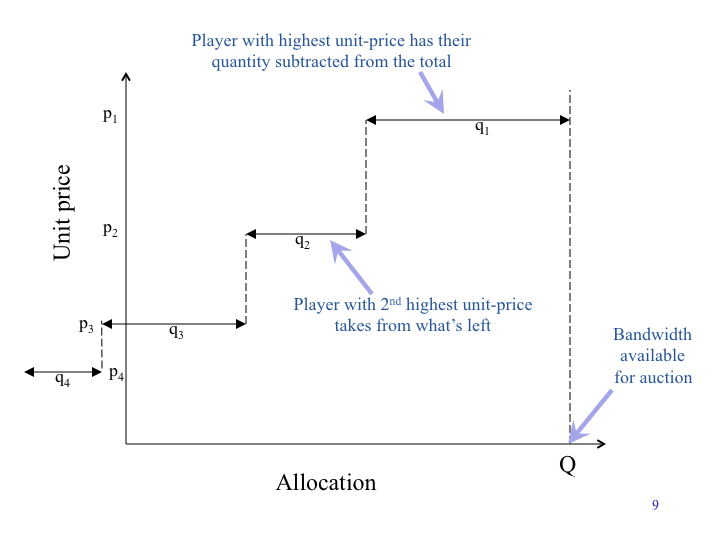
\includegraphics[width=0.8\textwidth]{allocation}
       \caption{The allocation procedure. The highest unit-price bidder is fully served, the second-highest is served from what's left, and so on. Bidders who bid too low are allocated zero bandwidth if it is all given to higher bidders.}
 \label{fig:allocation}
\end{figure}

The cost charged to a bidder is based on the 'exclusion compensation' principle, which extends the second-price principle. The fact that a given bidder {\it i} exists may mean that other bidders are not granted the same allocation they would have if bidder {\it i} were not participating. Bidder {\it i} therefore pays for the amount by which they inconvenience those other bidders. I.e. for all bidders other than {\it i} who receive an allocation when {\it i} doesn't participate, the change in their allocation with bidder {\it i} participating is multiplied by the unit-price they were willing to pay, and the sum is the cost charged to bidder {\it i}.

Figure~\ref{fig:cost} illustrates this.

\begin{figure}[h]
 \centering
   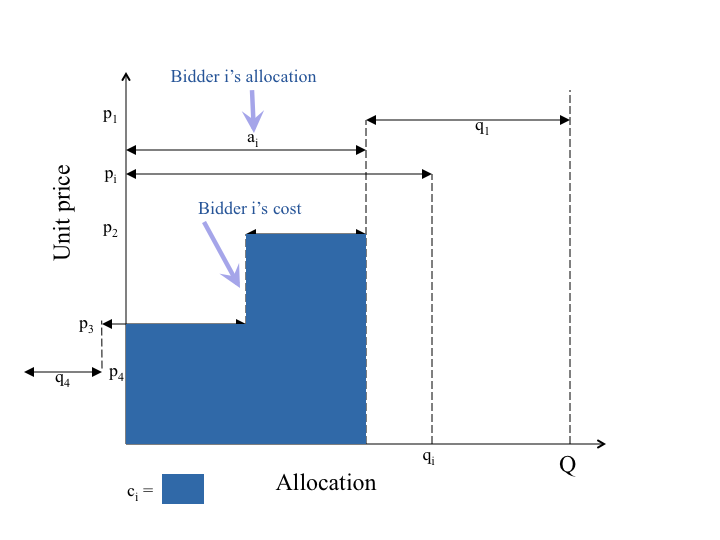
\includegraphics[width=0.8\textwidth]{cost}
       \caption{Calculating the cost.}
 \label{fig:cost}
\end{figure}

\section{The PSP on LHCONE}

The PSP as described works well for single network links, with a single divisible item auctioned among several bidders. However, LHCONE is a far more complex beast, as can be seen in figure~\ref{fig:lhcone}.

\begin{figure}[h]
 \centering
   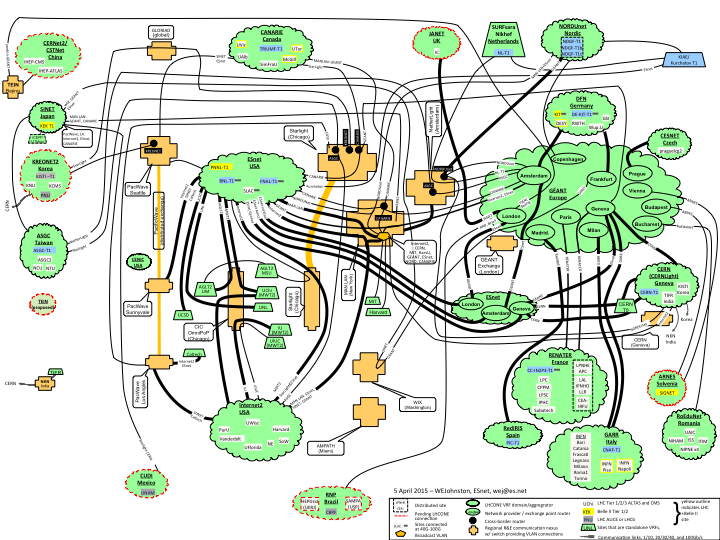
\includegraphics[width=0.8\textwidth]{LHCONE}
       \caption{An approximate schematic of the LHCONE network links, showing the complexity of the LHCONE layout.}
 \label{fig:lhcone}
\end{figure}

Fortunately, the PSP extends naturally to multiple links, where different bidders are interested in different network paths of the network. A full analysis is shown in \cite{PSP-multi}. The PSP properties are maintained by holding multiple independent auctions for each network link. Bidders have a global budget each, which again can vary from bidder to bidder, from which they bid on each of the links that they are interested in in parallel. The optimal strategy for a bidder is to bid for the same bandwidth on each link-segment of the network path they are interested in, varying the price they bid at each segment in accordance with the competition for that link. Convergence to an \textepsilon-Nash equilibrium is still guaranteed for rational bidders, making the PSP a viable candidate for addressing the problem of sharing bandwidth at LHCONE.

One issue that may arise in a complex topology like LHCONE is the existence of multiple paths between endpoints. Whether these are presented to the user as multiple routes on which they must bid, or are hidden inside the LHCONE representation, is an implementation detail, albeit a significant one. If the user is expected to bid on multiple paths for the same traffic then they obviously have a much more complex situation to handle, one which they would probably prefer not to have to deal with. On the other hand, if LHCONE attempts to hide the details of multi-path routing from the user, the maximum bandwidth available between any given pair of endpoints may not be constant, depending on other users on some of the paths.
\section{Conclusions}

blah blah blah
waffle waffle waffle
% \input{section-4-....tex}
% \input{section-4-....tex}
% \input{section-4-....tex}
% \input{section-4-....tex}

\par
\section*{References}

\begin{thebibliography}{1}

\bibitem{CompModel}
%  CMS computing : Technical Design Report {\it CERN-LHCC-2005-023}
  Grandi C, Stickland D and Taylor L 2005 The CMS Computing Model {\it CERN-LHCC-2004-35/G-083, CMS note 2004-031}

\bibitem{PhEDEx}
  Egeland R, Wildish T and Metson S 2008 Data transfer infrastructure for CMS data taking,  {\it XII Advanced Computing and Analysis Techniques in Physics Research (Erice, Italy: Proceedings of Science)}

\bibitem{PSP}

\bibitem{PSP-multi}

\end{thebibliography}


\end{document}
